\documentclass[sigconf]{acmart}

\usepackage{tikz}
\usetikzlibrary{positioning, shapes.geometric, arrows.meta, fit, backgrounds}
\definecolor{primaryblue}{HTML}{2B6CB0}
\definecolor{softblue}{HTML}{EBF8FF}
\definecolor{primarygreen}{HTML}{2F855A}
\definecolor{softgreen}{HTML}{F0FFF4}
\definecolor{darkgray}{HTML}{2D3748}
\definecolor{lightgray}{HTML}{EDF2F7}
\definecolor{accentorange}{HTML}{DD6B20}


%%
%% \BibTeX command to typeset BibTeX logo in the docs
\AtBeginDocument{%
  \providecommand\BibTeX{{%
    Bib\TeX}}}

%% Rights management information.  This information is sent to you
%% when you complete the rights form.  These commands have SAMPLE
%% values in them; it is your responsibility as an author to replace
%% the commands and values with those provided to you when you
%% complete the rights form.

% You may pick any of the following copyright options:
%\setcopyright{rightsretained}
\setcopyright{cc} % Creative Comments license


% You can pick the following creative comments license types (if \setcopyright{cc}):
% zero     % CC0 1.0 Universal
% by       % Attribution
% by-sa    % Attribution-ShareAlike
% by-nd    % Attribution-NoDerivatives
% by-nc    % Attribution-NonCommercial
% by-nc-sa % Attribution-NonCommercial-ShareAlike
% by-nc-nd % Attribution-NonCommercial-NoDerivatives
\setcctype{by}

\acmConference[MuC'26]{Mensch und Computer 2026 – Tagungsband, Gesellschaft für Informatik e.V.}{30. August - 02. September 2026}{Duisburg, Germany}
\acmDOI{10.18420/muc2026-mci-src-251}

%%
%% end of the preamble, start of the body of the document source.
\begin{document}

%%
%% The "title" command has an optional parameter,
%% allowing the author to define a "short title" to be used in page headers.
\title{Monitoring and Understanding Notebook-Based Learning with Jupyter} % [Short Title]
\subtitle{} % Only have this if your paper is written in a language other than English. 

%%
%% The "author" command and its associated commands are used to define
%% the authors and their affiliations.
%% Of note is the shared affiliation of the first two authors, and the
%% "authornote" and "authornotemark" commands
%% used to denote shared contribution to the research.

\settopmatter{authorsperrow=3}

\author{Arturo Olivares Martos}
\orcid{0009-0000-9415-7268}
\affiliation{%
  \institution{Universidad de Granada}
  \city{Granada}
  \country{Spain}}
\affiliation{%
  \institution{Universität Duisburg-Essen}
  \city{Duisburg}
  \country{Germany}}
\email{arturoolivares@correo.ugr.es}
\email{arturo.olivares@stud.uni-due.de}

\author{Lisa Pawlowski}
\orcid{0009-0006-5326-3180}
\affiliation{%
  \institution{Universität Duisburg-Essen}
  \city{Duisburg}
  \country{Germany}}
\email{lisa.pawlowski.99@stud.uni-due.de}

\author{Mohamed Abdelmagied}
\orcid{0009-0009-9692-7540}
\affiliation{%
  \institution{Universität Duisburg-Essen}
  \city{Duisburg}
  \country{Germany}}
\email{mohamed.abdelmagied@stud.uni-due.de}

\author{Kaimao Sheng}
\orcid{0009-0002-0639-6328}
\affiliation{%
  \institution{Universität Duisburg-Essen}
  \city{Duisburg}
  \country{Germany}}
\email{kaimao.sheng@uni-due.de}

\author{Irene-Angelica Chounta}
\orcid{0000-0001-9159-0664}
\affiliation{%
  \institution{Universität Duisburg-Essen}
  \city{Duisburg}
  \country{Germany}}
\email{irene-angelica.chounta@uni-due.de}



%%
%% By default, the full list of authors will be used in the page
%% headers. Often, this list is too long, and will overlap
%% other information printed in the page headers. This command allows
%% the author to define a more concise list
%% of authors' names for this purpose.
\renewcommand{\shortauthors}{Olivares Martos, Pawlowski, et al.}

%%
%% The abstract is a short summary of the work to be presented in the
%% article.
\begin{abstract}
As programming becomes increasingly integrated into scientific and educational workflows, the need to understand how users interact with computational notebooks has grown. This project introduces a JupyterLab dashboard extension that monitors and visualizes notebook activity, including notebook openings, cell execution outcomes, errors, and retries. The system produces summary statistics and visual timelines that portray how the workflow unfolds. The dashboard is intended to be used by students for self-assessment and awareness of their coding patterns. A survey was conducted to gather user feedback on the dashboard's usability and usefulness. The insights gained from this evaluation serve as a pilot study, establishing a baseline for the tool's usability and paving the way for future research on its pedagogical impact.
\end{abstract}


%% Comment the following if you do not write in German.
% \begin{translatedabstract}{german}
% Dies ist die Vorlage für Mensch und Computer 2026. \textbf{Note:} Only have this if your paper is written in a language other than English.
% \end{translatedabstract}


%%
%% The code below is generated by the tool at http://dl.acm.org/ccs.cfm.
%% Please copy and paste the code instead of the example below.
%%

\begin{CCSXML}
<ccs2012>
   <concept>
       <concept_id>10010405.10010489.10010491</concept_id>
       <concept_desc>Applied computing~Interactive learning environments</concept_desc>
       <concept_significance>500</concept_significance>
       </concept>
   <concept>
       <concept_id>10003120.10003145.10011769</concept_id>
       <concept_desc>Human-centered computing~Empirical studies in visualization</concept_desc>
       <concept_significance>500</concept_significance>
       </concept>
 </ccs2012>
\end{CCSXML}
\ccsdesc[500]{Applied computing~Interactive learning environments}
\ccsdesc[500]{Human-centered computing~Empirical studies in visualization}


%%
%% Keywords. The author(s) should pick words that accurately describe
%% the work being presented. Separate the keywords with commas.
\keywords{
  Jupyter Notebooks,
  Learning Analytics,
  Educational Dashboards,
  Student Self-Assessment,
  Instructor Insights,
  Interactive Coding Environments
}


%% A "teaser" image appears between the author and affiliation
%% information and the body of the document, and typically spans the
%% page.
%\begin{teaserfigure}
%  \includegraphics[width=\linewidth]{sampleteaser}
%  \caption{Seattle Mariners at Spring Training, 2010.}
%  \Description{Enjoying the baseball game from the third-base
%  seats. Ichiro Suzuki preparing to bat.}
%  \label{fig:teaser}
%\end{teaserfigure}

%%
%% This command processes the author and affiliation and title
%% information and builds the first part of the formatted document.
\maketitle

\section{Introduction}

This paper presents the design of a newly developed JupyterLab extension -- a learner-facing dashboard that tracks detailed notebook interactions, such as cell-level execution histories and error patterns, to support self-reflection in programming education.
Understanding the programming process is important because computational notebooks are central to modern data science education, yet instructors often lack visibility into how students work, and learners themselves rarely have opportunities to reflect on their own workflows, error patterns, or problem-solving behaviors~\cite{perkel2018jupyter, robinson2022error}.
Related research explores the use of learning dashboards to enhance students' self-awareness, foster reflection, and offer instructors actionable insights into learner behavior.
However, the majority of existing dashboards focus on high-level learning management system data rather than fine-grained programming behavior within computational notebooks~\cite{paulsen2024learning}.
To address this gap, we develop a student-centered dashboard extension in JupyterLab and evaluate its usability, perceived usefulness, and cognitive workload through an exploratory study with 22 students using standardized evaluation instruments (SUS, TAM, and NASA-TLX)~\cite{germanupa_sus, davis1989technology, hart1988development}.
In particular, we aim to answer the following research question: \textit{Whether the proposed dashboard extension is perceived by students as useful, easy to integrate into their workflow, and usable without imposing an excessive cognitive workload during programming tasks.}

This work has two contributions: 1) the design and implementation of a dashboard that captures programming behavior directly within JupyterLab, shifting focus from final code correctness to the learning process, and 2) empirical evidence on its acceptance, usability and cognitive impact, offering practical insights for building reflective tools in computational learning environments.


\section{Related Work}
Jupyter notebooks are widely used for scientific computing, data analysis, and programming education \cite{perkel2018jupyter}. Their combination of executable code, narrative text, and visual output supports exploratory and iterative work practices in which learners repeatedly test, revise, and interpret code. At the same time, programming learners often struggle with error identification and debugging, frequently relying on trial-and-error strategies \cite{robinson2022error}. Prior work on notebook-based analytics shows that cell-level traces such as execution patterns, time on task, and navigation behavior can reveal retries, hesitation, and fragmented workflows that remain invisible in final notebook submissions \cite{cai2025jupyter,JELAI}. Recent approaches to notebook analytics differ in their intended audience and purpose. Some systems provide infrastructures for collecting, analyzing, and visualizing distributed student activity, primarily to support instructors \cite{cai2025jupyter}. Other approaches analyze graded notebooks at assignment or course level to provide insights into performance and diversity \cite{groher2024learning}, combine fine-grained notebook traces with AI-supported tutoring \cite{JELAI}, or examine notebook changes retrospectively through repository histories \cite{raghunandan2023code}. More broadly, learner-facing dashboards must support students in interpreting visualizations and translating them into meaningful actions \cite{jivet2020students}, while their information design may also affect cognitive load \cite{cheng2024influence}. Compared with these approaches, our work focuses on embedding the system directly in JupyterLab and presenting live cell-level execution, error, retry, and focus-time information to students. The contribution therefore lies in a non-AI, learner-facing reflection interface and an initial learner-centered evaluation of its usability, perceived usefulness, ease of use, and workload.
%From an HCI perspective, such notebook activity can be understood as part of broader sensemaking processes, in which users iteratively annotate, branch, document, and revise computational work \cite{raghunandan2023code}.

Learning dashboards have been discussed as tools for supporting awareness, reflection, and self-regulated learning \cite{schwendimann2016perceiving,corrin2014exploring}. However, many existing dashboards rely on coarse-grained learning management system data, such as resource access, assignment completion, or overall activity patterns, which limits their ability to represent the step-by-step nature of programming work \cite{paulsen2024learning}. %Human-centered perspectives on learning analytics emphasize that dashboards should not be designed around data availability alone, but around users' needs, contexts, and interpretation processes \cite{chejara2024human}. %This is particularly relevant for programming education, where dashboard visualizations need to be understandable and actionable within an already complex coding environment.
Existing approaches in programming education often remain instructor-facing, assignment-level, or performance-oriented, rather than supporting student-directed reflection on fine-grained coding behavior \cite{sondagar2021elearning,groher2024learning}. For learner-facing dashboards, the central challenge is not only to visualize activity data, but to support students' sense-making and actionability. \cite{jivet2020students} show that students' interpretation of dashboard visualizations depends on factors such as transparency of design, reference frames, and support for action. In addition, dashboard information design may affect cognitive load and learning performance, making workload an important evaluation dimension \cite{cheng2024influence}. %Taken together, prior work suggests a gap in understanding how students perceive fine-grained, learner-facing visualizations of notebook-based programming behavior in terms of usability, usefulness, and workload. The present study addresses this gap by designing and evaluating a JupyterLab dashboard that visualizes cell-level interaction data to support student self-reflection.

%\section{Methodology}
\section{Dashboard Design and Implementation}
\begin{figure}
    \centering
    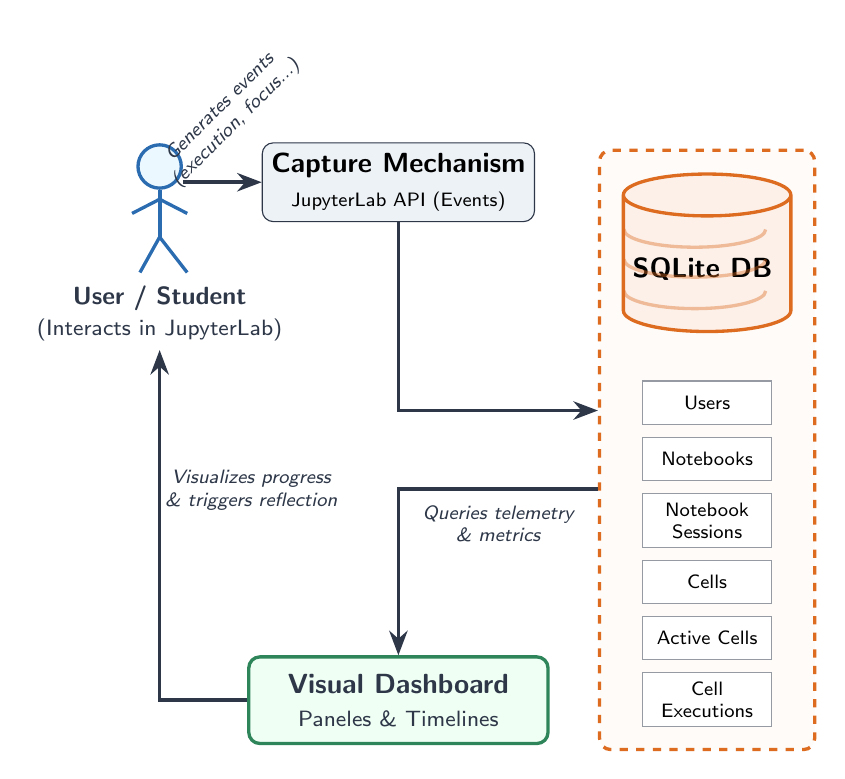
\begin{tikzpicture}[
        font=\sffamily,
        >=Stealth,
        % Reduced horizontal spacing significantly to save width
        node distance=1.4cm and 1.2cm,
        % Dashboard block style
        dashblock/.style={
            rectangle, 
            draw=primarygreen, 
            fill=softgreen, 
            rounded corners, 
            minimum width=3.8cm, 
            minimum height=1.1cm, 
            align=center, 
            line width=1.2pt,
            text=darkgray
        },
        % Database tables style (Compact width)
        tableblock/.style={
            rectangle, 
            draw=darkgray!50, 
            fill=white, 
            minimum width=1.4cm, 
            minimum height=0.55cm, 
            align=center, 
            text width=1.4cm,
            font=\sffamily\scriptsize
        },
        % Database main icon (Cylinder)
        % Database main icon (Realistic 3D Cylinder with elliptical top)
        dbshape/.style={
            cylinder, 
            draw=accentorange, 
            fill=accentorange!10, 
            shape border rotate=90, 
            aspect=0.25, % Creates a realistic 3D ellipse on top
            minimum width=1.8cm, 
            minimum height=2cm, 
            line width=1.2pt, 
            align=center
        },
        % Flow arrows style
        flow/.style={
            draw=darkgray, 
            ->, 
            line width=1.3pt
        },
        % Flow labels style
        flowtext/.style={
            font=\sffamily\scriptsize\itshape, 
            align=center, 
            text=darkgray
        }
    ]
    
        % ==========================================
        % 1. USER REPRESENTATION (Stickman)
        % ==========================================
        \begin{scope}[local bounding box=userbox]
            % Head
            \node[circle, draw=primaryblue, fill=softblue, minimum size=0.55cm, line width=1.2pt] (head) at (0,0) {};
            % Torso
            \draw[primaryblue, line width=1.5pt] (head.south) -- ++(0,-0.6) coordinate (torso);
            % Arms
            \draw[primaryblue, line width=1.2pt] (head.south)++(0,-0.12) -- ++(-0.35,-0.18);
            \draw[primaryblue, line width=1.2pt] (head.south)++(0,-0.12) -- ++(0.35,-0.18);
            % Legs
            \draw[primaryblue, line width=1.2pt] (torso) -- ++(-0.25,-0.45);
            \draw[primaryblue, line width=1.2pt] (torso) -- ++(0.35,-0.45);
            % Label below the legs
            \node[below=0.5cm of torso, font=\sffamily\bfseries\small, text=darkgray, align=center] {User / Student\\ \mdseries\footnotesize(Interacts in JupyterLab)};
        \end{scope}
    
        % ==========================================
        % 2. CAPTURE MECHANISM (Middle-Left)
        % ==========================================
        % Reduced right distance from 2.6cm to 1.2cm to bring it closer to the user
        \node[rectangle, draw=darkgray, fill=lightgray, rounded corners, right=1cm of head, yshift=-0.2cm, minimum width=3.2cm, minimum height=1.0cm, align=center] (api) {
            \textbf{Capture Mechanism} \\ 
            \scriptsize{JupyterLab API (Events)}
        };
    
        % ==========================================
        % 3. DATABASE STRUCTURE (Cylinder + Vertically Stacked Tables)
        % ==========================================
        \node[dbshape, right=1.1cm of api, yshift=-1.1cm] (sqlite) {
            \textbf{SQLite DB}
        };
    
        % Subtle segment lines inside the SQLite DB cylinder (elliptical arcs)
        \draw[accentorange, opacity=0.4, line width=1.2pt] 
            ([yshift=0.12cm, xshift=0.8pt]sqlite.west) arc (180:360:0.9cm and 0.225cm);
        \draw[accentorange, opacity=0.4, line width=1.2pt] 
            ([yshift=-0.28cm, xshift=0.8pt]sqlite.west) arc (180:360:0.9cm and 0.225cm);
            \draw[accentorange, opacity=0.4, line width=1.2pt] 
            ([yshift=0.5cm, xshift=0.8pt]sqlite.west) arc (180:360:0.9cm and 0.225cm);
    
        % Stacked tables in a single vertical column to minimize width
        \node[tableblock, below=0.6cm of sqlite] (t1) {Users};
        \node[tableblock, below=0.15cm of t1] (t2) {Notebooks};
        \node[tableblock, below=0.15cm of t2] (t3) {Notebook Sessions};
        \node[tableblock, below=0.15cm of t3] (t4) {Cells};
        \node[tableblock, below=0.15cm of t4] (t5) {Active Cells};
        \node[tableblock, below=0.15cm of t5] (t6) {Cell Executions};
    
        % Background container bounding the DB structure
        \begin{scope}[on background layer]
            \node[draw=accentorange, dashed, line width=1.2pt, fill=accentorange!3, rounded corners, inner sep=8pt, fit=(sqlite) (t1) (t6)] (dbcontainer) {};
        \end{scope}
    
        % ==========================================
        % 4. VISUALIZATION DASHBOARD
        % ==========================================
        \node[dashblock, below=5.5cm of api] (dash) {
            \textbf{Visual Dashboard} \\ 
            \footnotesize{Paneles \& Timelines}
        };
    
        % ==========================================
        % DATA FLOWS & CONNECTIONS
        % ==========================================
        
        % From User to Capture API (Label rotated 45 degrees to fit tightly between nodes)
        \path[flow] ([yshift=-0.2cm]head.east) -- node[flowtext, rotate=45, above, pos=1, yshift=0.5cm, xshift=0.3cm] {Generates events \\ (execution, focus...)} (api.west);
        
        % From API to SQLite Database (Enters exactly 0.5cm above the west center)
        \path[flow] (api.south) |- ([yshift=0.5cm]dbcontainer.west);
        
        % From Database to Visual Dashboard (Leaves exactly 0.5cm below the west center -> 1.0cm gap)
        \path[flow] ([yshift=-0.5cm]dbcontainer.west) -| node[flowtext, below, pos=0.25, yshift=-2pt] {Queries telemetry \\ \& metrics} (dash.north);
        
        % Feedback loop: from Dashboard back to the User
        \path[flow] (dash.west) -| node[flowtext, right, pos=0.8, xshift=-2pt] {Visualizes progress \\ \& triggers reflection} (userbox.south);
    
    \end{tikzpicture}
    \Description{A conceptual architecture diagram showing the data flow of the JupyterLab learning analytics system. It consists of four main parts arranged in a loop. On the left, a stickman icon represents the ``User / Student (Interacts in JupyterLab)''. An arrow points from the user's head to a light grey box in the middle labeled ``Capture Mechanism (JupyterLab API (Events))'' with the text ``Generates events (execution, focus...)'' rotated at 45 degrees. From the bottom of the Capture Mechanism, a right-angled arrow goes to the right, entering a large orange dashed box representing the Relational Storage. Inside this storage, there is an orange 3D cylinder representing the ``SQLite DB'' (divided into three stacked segments by subtle internal lines) and a vertical column of six white tables: ``Users'', ``Notebooks'', ``Notebook Sessions'', ``Cells'', ``Active Cells'', and ``Cell Executions''. From the left side of the Relational Storage container, a right-angled arrow labeled ``Queries telemetry \& metrics'' points down to a green box at the bottom center labeled ``Visual Dashboard (Paneles \& Timelines)''. Finally, an arrow labeled ``Visualizes progress \& triggers reflection'' goes from the left side of the Dashboard back up to the student, closing the continuous feedback loop.}
    \caption{Data flow architecture of the learner-facing dashboard: telemetry events are captured from user interactions via the JupyterLab API, persisted into the SQLite relational database, and queried to render reflective visualizations.}
    \label{fig:data_flow_architecture}
\end{figure}
Our learner-facing dashboard extension is designed to help students reflect on their work and identify learning gaps during programming tasks within JupyterLab. A video demo of our extension can be found \href{https://www.youtube.com/watch?v=VZKJdUi2B-k}{\color{blue}\underline{here}}, and the data flow architecture is represented in Figure~\ref{fig:data_flow_architecture}.
\subsection{Data Collection Mechanism}

Using JupyterLab's API~\cite{jupyterlab_tutorial_2024, jupyterlab_extension_template}, the tool monitors active sessions and logs telemetry events in a relational SQLite database containing six core tables:
\begin{description}
    \item[Users] Stores anonymous personal codes and roles (student/teacher\footnote{The teacher role is there for potential future use.}). %The code is only used to link the data collected from the JupyterLab extension to the survey responses.
    
    \item[Notebooks] Tracks notebook metadata (title, path, author).
    
    \item[Notebook Sessions] Captures timestamps for when notebooks are opened and closed and by whom.
    
    \item[Cells] Logs cell types (code, markdown, raw) and original content.
    
    \item[Active Cells] Monitors active user focus with exact interaction durations.
    
    \item[Cell Executions] Tracks code execution metrics, runtime outputs, and error counts/messages.
\end{description}

\subsection{Data Visualization Panels}

\begin{figure}
    \centering
    
\includegraphics[width=0.85\linewidth]{img/Dashboard/Dashboard_Part1.png}
    \caption{The upper section of the learner-facing JupyterLab dashboard.}
    \Description{A screenshot of the upper half of the JupyterLab dashboard interface. At the top, a header displays the anonymous user ID NAMA1968 and the access level designated as Student. Below this, the Current Progress panel shows a progress bar indicating 38 percent completion. The Success/Error/Attempt Rate panel displays a horizontal bar chart segmented into 13 percent green for single-attempt success, 25 percent yellow for multiple attempts, and 25 percent red for final errors. The Error Rate panel features a circular donut chart showing a 33 percent error rate. At the bottom, the Top Error Cells panel lists code cells with execution failures, showcasing a specific cell containing a Python tuple with a red badge indicating 4 fails.}
    \label{fig:dashboard_part1}
\end{figure}
\begin{figure}
    \centering
    
\includegraphics[width=0.85\linewidth]{img/Dashboard/Dashboard_Part2.png}
    \caption{The lower section of the learner-facing JupyterLab dashboard.}
    \Description{A screenshot of the lower half of the JupyterLab dashboard interface. It starts with the Top Time-Consuming Cells panel, listing two specific Python cells: one showing an active focus time of 10 minutes and 24 seconds, and another showing 10 seconds. Below, the Top Common Error Types panel presents a bar graph ranking errors, showing IndexError with 3 occurrences, followed by SyntaxError and NameError with 1 occurrence each. At the bottom, the Execution Timeline displays two horizontal dashed lines with chronologically ordered green and red dots representing successful and failed cell executions over time.}
    \label{fig:dashboard_part2}
\end{figure}

The user interface (Figures~\ref{fig:dashboard_part1} and~\ref{fig:dashboard_part2}), accessible through the JupyterLab command palette, is organized into distinct panels\footnote{The dashboard visualization is available \href{https://git.uni-due.de/colaps/la-rp/group-4/la-extension/-/raw/master/MUC\%20-\%20StudentResearchCompetition/Dashboard/Dashboard.pdf?ref_type=heads&inline=true}{\color{blue}\underline{here}}.} (each featuring a ``Help'' button for interpretation):
\begin{description}
    \item[User Information] Displays the user's anonymous ID code and role.

    \item[Current Progress] Shows a percentage metric tracking error-free code execution according to Equation~\eqref{eq:progress}.
    \begin{equation}\label{eq:progress}
        \text{Progress} = \frac{\text{Code cells with an execution without errors}}{\text{Total number of code cells}}
        \times 100\%
    \end{equation}

    \item[Success/Error/Attempt Rate] Classifies cells into three status categories and shows the rate of each category:
    \begin{itemize}
        \item \emph{Successful}: Single execution, zero errors.
        \item \emph{Attempted}: Multiple executions, but the final attempt was successful.
        \item \emph{Error}: The final execution resulted in a failure.
    \end{itemize}

    \item[Error Rate] Displays overall execution failure rates using a dynamic color gradient scale (0\% green to 100\% red) according to Equation~\eqref{eq:error_rate}.
    \begin{equation}\label{eq:error_rate}
        \text{Error Rate} = \frac{\text{Number of executions with errors}}{\text{Total number of executions}}
        \times 100\%
    \end{equation}

    \item[Top Error Cells] Lists the top $n$ cells with the most failed executions, including a jump-to-cell navigation link.

    \item[Top Attempt Cells] Highlights the top $n$ cells requiring the highest volume of total executions.

    \item[Top Time-Consuming Cells] Ranks cells by total time active during the workspace session.

    \item[Top Common Error Types] Tallies occurrences of specific Python exceptions (e.g., \texttt{SyntaxError}, \texttt{NameError}).

    \item[Execution Timeline] A chronologically plotted dot graph of executions, color-coded by outcome (green for success, red for errors) to illustrate workflow trends over time.
\end{description}

The dashboard metrics are intended as reflection cues rather than diagnostic measures of programming ability or learning. A high error rate or recurring error type may encourage students to inspect the corresponding messages and revisit the underlying concept. Repeated executions may prompt learners to review their current strategy or test their code in smaller steps, while time-consuming cells may indicate points where task decomposition or additional support could be helpful. However, these patterns can have multiple explanations such as repeated executions which also reflect productive experimentation, and long active times which represent deliberate work rather than difficulty. The \emph{Help} function therefore explains each metric, provides a cautious interpretation, and suggests possible next actions.

\section{Evaluation}

To evaluate how students experience the dashboard as a learner-facing reflection interface, we conducted an exploratory, cross-sectional user study. The aim was to assess students' perceptions of the dashboard in terms of usability, perceived usefulness, ease of use, and workload. Twenty-two (22) students participated in the study and interacted with the dashboard while solving Python exercises in JupyterLab. Participants differed in their prior experience with Jupyter Notebook and Python, allowing the dashboard to be evaluated by learners with varying programming backgrounds.

The study was approved by the Ethics Committee of the Faculty of Computer Science at the University of Duisburg-Essen\footnote{Ethics certificate ID: 2601CMPL2910.}. After providing informed consent, participants first answered background questions on their previous experience with Jupyter Notebook and Python. They then used the JupyterLab dashboard during a programming task and subsequently completed standardized post-use questionnaires\footnote{Questionnaires are available \href{https://git.uni-due.de/colaps/la-rp/group-4/la-extension/-/raw/master/MUC\%20-\%20StudentResearchCompetition/Questionaire.pdf?ref_type=heads&inline=true}{\color{blue}\underline{here}}.}. Usability was measured with the System Usability Scale (SUS), a ten-item instrument resulting in a score from 0 to 100 \cite{germanupa_sus}. Perceived usefulness and perceived ease of use were assessed using items based on the Technology Acceptance Model (TAM) \cite{davis1989technology}. Subjective workload was measured with the NASA Task Load Index (NASA-TLX), covering mental demand, physical demand, temporal demand, perceived performance, effort, and frustration \cite{hart1988development}.

The collected data were analyzed descriptively to summarize students' perceptions of the dashboard. In addition, Spearman rank correlations were computed exploratively to examine relationships between usability, perceived usefulness, ease of use, and workload. This evaluation provides an initial empirical basis for understanding whether fine-grained notebook visualizations can be integrated into students' programming workflows without imposing excessive cognitive burden.

\section{Results}
The final sample consisted of 22 students with varying prior experience in Jupyter Notebook and Python. On average, participants spent about 17 minutes testing the dashboard while solving Python exercises. All multi-item scales showed acceptable to excellent internal consistency (SUS: $\alpha=.794$; PU: $\alpha=.852$; PEOU: $\alpha=.941$). Descriptive statistics are reported in Table~\ref{tab:descriptive_stats}.

\begin{table}
  \centering
  \caption{Descriptive Statistics of Main Evaluation Measures ($N=22$)}
  \label{tab:descriptive_stats}
  \small
  \begin{tabular}{l r r r r}
    \toprule
    \textbf{Measure} & \textbf{M} & \textbf{SD} & \textbf{Min} & \textbf{Max} \\
    \midrule
    System Usability Scale (SUS)      & 65.57 & 17.89 & 40.00 & 90.00 \\
    TAM Overall                       &  5.36 &  0.88 &  3.25 &  6.75 \\
    \quad Perceived Usefulness (PU)   &  4.93 &  1.18 &  3.33 &  7.00 \\
    \quad Perceived Ease of Use (PEOU)&  5.78 &  1.06 &  3.17 &  7.00 \\
    NASA-TLX                          &  8.15 &  2.92 &  1.67 & 12.67 \\
    \bottomrule
  \end{tabular}
\end{table}

The mean SUS score (65.57) fell just below the common benchmark of 68, indicating generally usable but improvable interface design; presenting multiple fine-grained indicators at once may have raised perceived complexity for some users.

Technology acceptance was positive overall (TAM $M=5.36$ on a seven-point scale), but Perceived Ease of Use exceeded Perceived Usefulness ($5.78$ vs.\ $4.93$). Students thus found the dashboard easy to operate, while its immediate value for self-reflection was less evident. Qualitative comments echoed this: some participants saw the dashboard as more useful for instructors, or asked for more actionable support such as guidance on resolving specific errors.

Subjective workload was low to moderate (NASA-TLX $M=8.15$ on a 0--20 scale), suggesting the dashboard did not impose excessive cognitive burden. Together, these results indicate that fine-grained notebook visualizations can be integrated into students' workflows in a usable, low-workload manner, but that their reflective value depends on stronger interpretive and actionable support.

\section{Conclusions}
This study presented and evaluated a learner-facing JupyterLab dashboard that visualizes fine-grained notebook interactions to support students' reflection on their programming processes. The results suggest these visualizations can be integrated into notebook-based workflows with good usability and low workload: students found the dashboard relatively easy to use and did not report excessive cognitive burden, though they rated its usefulness for self-reflection more moderately. Visibility is thus only the first step. Learners also need support in interpreting the information and translating it into concrete next steps. This work contributes an initial learner-centered evaluation of fine-grained notebook visualizations as reflection interfaces in programming education. This exploratory study has several limitations. The evaluation involved 22 students who interacted with the dashboard for approximately 17 minutes. The cross-sectional post-use design captures participants' perceived usability, usefulness, ease of use, and workload after short-term use, but it does not establish whether the dashboard improves self-reflection, debugging behavior, programming strategies, or learning outcomes. The findings should therefore be interpreted as initial evidence of short-term user experience rather than pedagogical effectiveness. Future longitudinal or controlled studies should examine how students use the dashboard over time and whether it leads to changes in programming behavior and learning.

%%
%% The acknowledgments section is defined using the "acks" environment
%% (and NOT an unnumbered section). This ensures the proper
%% identification of the section in the article metadata, and the
%% consistent spelling of the heading.
% \begin{acks}
% To Robert, for the bagels and explaining CMYK and color spaces.
% \end{acks}

%%
%% The next two lines define the bibliography style to be used, and
%% the bibliography file.
\bibliographystyle{ACM-Reference-Format}
\bibliography{bibliography}


%%
%% If your work has an appendix, this is the place to put it.
%\appendix
%\section{Research Methods}


\end{document}
\endinput
%%
%% End of file `sample-manuscript.tex'.
